\problemname{\problemyamlname}

%\illustration{0.3}{image.jpg}{Caption of the illustration (optional). CC BY-NC 2.0 by X on Y}
% Source: URL to image.

% optionally define variables/limits for this problem
In preparation for the next edition of the BAPC at UCLouvain, KARWa Corp. wishes to connect all the karaokes of Belgium with eachother.
For that, they contact the SNCB and the STIB who call you to find the best way to connect all the karaokes.

There are $n$ karaokes numbered from $1$ to $n$ and $m$ bidirectional connections between some of them.
Each connection has a weight $w$ representing the distance between all the connected karaokes.
The goal is to connect all the karaokes between them while minimizing the total cost (distance) of all the connections.

However, the small connections (with a small weight) are expensive, so the SNCB wishes to maximize the weight of the minimum edge such that the total cost (distance) of the connections is inferior to $125\%$ of the minimum cost (of the distance) to connect all the karaokes.
In other words. the total cost of the connections must be less than or equal to $1.25$ times the minimum cost for the project to be viable.

It is guaranteed that it's possible to connect all the karaokes between eachother.

\begin{figure}[h]
	\centering
	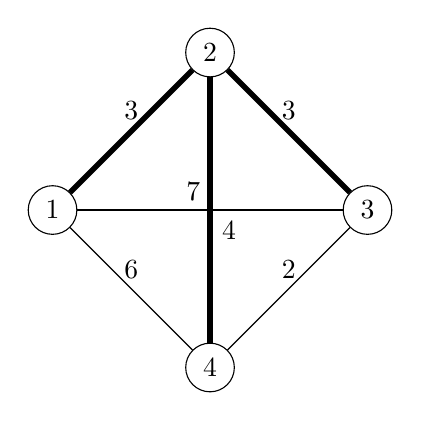
\begin{tikzpicture}
		% Définition des noeuds
		\node[circle,draw] (1) at (0,0) {1};
		\node[circle,draw] (2) at (2,2) {2};
		\node[circle,draw] (3) at (4,0) {3};
		\node[circle,draw] (4) at (2,-2) {4};
		
		% Définition des arêtes
		\draw (1) -- node[above]{6} (4);
		\draw[line width=2pt] (1) -- node[above]{3} (2);
		\draw[line width=2pt] (2) -- node[above]{3} (3);
		\draw (3) -- node[above]{2} (4);
		\draw[line width=2pt] (4) -- node[below right]{4} (2);
		\draw (1) -- node[above left]{7} (3);
	\end{tikzpicture}
	  \caption[]{Example 1, the network is bold}
\end{figure}

\begin{Input}
	The input consists of:
	\begin{itemize}
		\item One line with 2 integers $n$ and $m$ ($2 \le n \le 10^5$ and $1 \le m \le 2 \times 10^5$), representing respectively the number of karaokes and the number of connections between two karaokes.
		\item $m$ lines with 3 integers $u$, $v$ and $w$ ($1 \le u \le n$, $1 \le v \le n$ and $1 \le w \le 10^9$), representing a bidirectional connection between two karaokes $u$ and $v$ who's weight is $w$.
	\end{itemize}
\end{Input}

\begin{Output}
	An integer $k$ representing the weight of the minimum weight edge of the network which connects all the karaokes with a cost inferior to $125\%$ of the original cost.
\end{Output}
